%!TEX program = xelatex
\documentclass[11pt,a4paper]{article}
\usepackage[utf8]{inputenc}
\usepackage[T1]{fontenc}
\usepackage{authblk}
\usepackage{ctex}
\usepackage{tikz}
\usepackage{pgfplots}
\usepackage{verbatim}
\usepackage{amsfonts}
\usepackage{amsmath}
\usepackage{amsthm}
\usepackage{indentfirst}
\usepackage{amssymb}
\setlength{\parindent}{0pt}
\usetikzlibrary{shapes,snakes}
\newcommand{\argmax}{\operatornamewithlimits{argmax}}
\newcommand{\argmin}{\operatornamewithlimits{argmin}}
\DeclareMathOperator{\col}{col}
\usepackage{booktabs}
\newtheorem{theorem}{Theorem}
\newtheorem{note}{Note}
\newtheorem{definition}{Definition}
\newtheorem{proposition}{Proposition}
\newtheorem{lemma}{Lemma}
\newtheorem{example}{Example}
\newtheorem{corollary}{Corollary}
\usepackage{graphicx}
\usepackage{geometry}
\usepackage{hyperref}
\newcommand{\code}{	exttt}
\geometry{a4paper,scale=0.8}
\title{STAT R note}
\author[*]{Wenxiao Yang}
\affil[*]{Department of Mathematics, University of Illinois at Urbana-Champaign}
\date{2021}


\usepackage{listings}
\usepackage{xcolor}

\lstset{numbers=left,numberstyle=\tiny,keywordstyle=\color{blue},commentstyle=\color[cmyk]{1,0,1,0},frame=single,escapeinside=``,extendedchars=false,xleftmargin=2em,xrightmargin=2em,aboveskip=1em,tabsize=4,showspaces=false}






\begin{document}
\maketitle
\tableofcontents
\newpage

\section{Basic}
\subsection{读取数据 txt (galton)}
\begin{lstlisting}[language=R]
galton <- read.table("Galton.txt", header=TRUE)
\end{lstlisting}
\subsection{读取数据 csv (bikeshares)}
\begin{lstlisting}[language=R]
bikeshares <-  read.csv("BikeShares.csv", header=TRUE)
\end{lstlisting}
\subsection{查看数据维度 (bikeshares)}
\begin{lstlisting}[language=R]
dim(bikeshares)
## [1] 17414    10
\end{lstlisting}

\subsection{数据中删除列 (bikeshares)}
\begin{lstlisting}[language=R]
# We remove columns 1,  7, 8, 9, 10:
bikeshares.reg = bikeshares[,c(-1,-7,-8,-9,-10)] #-i即删除i列
head(bikeshares.reg)
##   cnt  t1  t2   hum wind_speed
## 1 182 3.0 2.0  93.0        6.0
## 2 138 3.0 2.5  93.0        5.0
## 3 134 2.5 2.5  96.5        0.0
## 4  72 2.0 2.0 100.0        0.0
## 5  47 2.0 0.0  93.0        6.5
## 6  46 2.0 2.0  93.0        4.0
\end{lstlisting}


\subsection{数据“列”处理:赋值,条件选中 (galton)}
\begin{lstlisting}[language=R]
# Define the Adjusted Heigth Variable (according to Galton)
galton$AH <- galton$Height
galton$AH[galton$Gender=="F"]<-galton$Height[galton$Gender=="F"]*1.08
galton$MP <- (galton$Father + 1.08*galton$Mother)/2
head(galton)
##   Family Father Mother Gender Height Kids     AH    MP
## 1      1   78.5   67.0      M   73.2    4 73.200 75.43
## 2      1   78.5   67.0      F   69.2    4 74.736 75.43
## 3      1   78.5   67.0      F   69.0    4 74.520 75.43
## 4      1   78.5   67.0      F   69.0    4 74.520 75.43
## 5      2   75.5   66.5      M   73.5    4 73.500 73.66
## 6      2   75.5   66.5      M   72.5    4 72.500 73.66
\end{lstlisting}

\subsection{查看数据类型 (bikeshare)}
\begin{lstlisting}[language=R]
class(numeric(n.iter))
## [1] "numeric"
class(bikeshares.reg)
## [1] "data.frame"
\end{lstlisting}


\subsection{data.frame}
\subsubsection{修改列名}
\begin{lstlisting}[language=R]
names(myCR) = c("t1","hum");
\end{lstlisting}
\subsubsection{data.frame列拼接cbind() (bikeshares)}
\begin{lstlisting}[language=R]
bikeshare.mlr1$fitted[1:5]
## 1         2         3         4         5 
## 158.12967 152.85747  42.50091 -77.95731 126.47427 
bikeshare.mlr1$residuals[1:5]
## 1         2         3         4         5 
## 23.87033 -14.85747  91.49909 149.95731 -79.47427 
cbind(bikeshare.mlr1$fitted[1:5], bikeshare.mlr1$residuals[1:5])
##        [,1]      [,2]
## 1 158.12967  23.87033
## 2 152.85747 -14.85747
## 3  42.50091  91.49909
## 4 -77.95731 149.95731
## 5 126.47427 -79.47427
\end{lstlisting}
\subsubsection{data.frame行拼接rbind() (bikeshares)}
\begin{lstlisting}[language=R]
rbind(bikeshare.mlr1$fitted[1:5], bikeshare.mlr1$residuals[1:5])
## 1         2        3         4         5
## [1,] 158.12967 152.85747 42.50091 -77.95731 126.47427
## [2,]  23.87033 -14.85747 91.49909 149.95731 -79.47427
\end{lstlisting}
\subsubsection{data.frame抽样}
\begin{lstlisting}[language=R]
head(bikeshares.reg)
##      cnt t1  t2  hum     wind_speed
## 1	182	3.0	2.0	93.0	6.0
## 2	138	3.0	2.5	93.0	5.0
## 3	134	2.5	2.5	96.5	0.0
## 4	72	2.0	2.0	100.0	0.0
## 5	47	2.0	0.0	93.0	6.5
## 6	46	2.0	2.0	93.0	4.0
bikeshares.reg[sample(5), c(3,4)] #前五行(第3,4列)中随机抽样
##      t2  hum
## 2	2.5	93.0
## 5	0.0	93.0
## 3	2.5	96.5
## 1	2.0	93.0
## 4	2.0	100.0
\end{lstlisting}

\subsection{集体求均值}
\begin{lstlisting}[language=R]
apply(bikeshares.reg,2,mean)
## cnt         t1         t2        hum wind_speed 
## 1143.10164   12.46809   11.52084   72.32495   15.91306 
\end{lstlisting}





\subsection{numeric}
\subsubsection{numeric(k): 生成k个0的numeric}
\begin{lstlisting}[language=R]
numeric(5)
## [1] 0 0 0 0 0
class(numeric(5))
## [1] "numeric"
\end{lstlisting}
\subsubsection{numeric 数值修改}
\begin{lstlisting}[language=R]
A=numeric(5)
A[1]=2
A
## [1] 2 0 0 0 0
\end{lstlisting}
\subsection{matrix}
\subsubsection{data.frame 转成 matrix}
\begin{lstlisting}[language=R]
M=data.matrix(X)
\end{lstlisting}

\subsubsection{修改列名}
\begin{lstlisting}[language=R]
colnames(x)=c("t1", "t2", "hum")
\end{lstlisting}

\subsubsection{去掉矩阵 列/行 的名字}
\begin{lstlisting}[language=R]
rownames(A)<-NULL
colnames(A)<-NULL
\end{lstlisting}

\subsubsection{自己创建matrix}
\begin{lstlisting}[language=R]
A=matrix(1:12,nrow=3,ncol=4)
A
##      [,1] [,2] [,3] [,4]
## [1,]    1    4    7   10
## [2,]    2    5    8   11
## [3,]    3    6    9   12
\end{lstlisting}
\subsubsection{Transpose of matrix 转置矩阵}
\begin{lstlisting}[language=R]
t(A)
##       [,1] [,2] [,3]
## [1,]    1    2    3
## [2,]    4    5    6
## [3,]    7    8    9
## [4,]   10   11   12
\end{lstlisting}
\subsubsection{Multiplication of matrix 矩阵乘法}
\begin{lstlisting}[language=R]
A%*%t(A)
##     [,1] [,2] [,3]
## [1,]  166  188  210
## [2,]  188  214  240
## [3,]  210  240  270
\end{lstlisting}
\subsubsection{解$Ax=b$: solve(A,b)}
Solve $ax=b$
\begin{lstlisting}[language=R]
A.data=data.frame(a=c(1,43,765,9),b=c(2,455,787,2),
                c=c(213,434,67,24),d=c(672,332,7,123))
A=data.matrix(A.data)
b=matrix(c(1,10,8,9))
solve(A,b)
##      [,1]
## a -0.6723499
## b  0.7380811
## c -0.9034118
## d  0.2866412
\end{lstlisting}

\subsubsection{矩阵行列式 : det()}
\begin{lstlisting}[language=R]
det(A)
\end{lstlisting}
\subsubsection{生成对角阵:diag(1,2,3,4)}
\begin{lstlisting}[language=R]
diag(c(1,2,3,4))
##     [,1] [,2] [,3] [,4]
## [1,]    1    0    0    0
## [2,]    0    2    0    0
## [3,]    0    0    3    0
## [4,]    0    0    0    4
\end{lstlisting}
\subsubsection{提取对角线上的元素:diag()}
\begin{lstlisting}[language=R]
diag(A)
## [1]   1 455  67 123
\end{lstlisting}
\subsubsection{特征值和特征向量:eigen()}
\begin{lstlisting}[language=R]
eigen(A)
## eigen() decomposition
## $values
## [1]  962.54862 -533.15335  195.96895   20.63578
## 
## $vectors
##             [,1]        [,2]       [,3]       [,4]
## [1,] -0.18050353 -0.31476395  0.7098847  0.5218457
## [2,] -0.65689212 -0.36245740 -0.6561850 -0.5428550
## [3,] -0.73165231  0.87683413  0.2141936  0.6319310
## [4,] -0.02441547 -0.02664961  0.1400217 -0.1834356
\end{lstlisting}

\subsubsection{逆矩阵 solve(A)}
\begin{lstlisting}[language=R]
solve(A)
##      [,1]          [,2]          [,3]        [,4]
## [1,]  0.015470466 -0.0038533021  0.0023771584 -0.07425607
## [2,] -0.016656510  0.0038972675 -0.0011449021  0.08054712
## [3,]  0.019498924 -0.0018420827  0.0012737127 -0.10163107
## [4,] -0.004665816  0.0005780095 -0.0004038514  0.03208420
\end{lstlisting}




\section{Simple Linear Regression}
\subsection{拟合slr (galton)}
\begin{lstlisting}[language=R]
# Simple Linear Regression
slr.fit <- lm(AH ~ MP, data=galton)
summary(slr.fit)
## 
## Call:
## lm(formula = AH ~ MP, data = galton)
## 
## Residuals:
##     Min      1Q  Median      3Q     Max 
## -9.4947 -1.4779  0.0995  1.5175  9.1262 
## 
## Coefficients:
##             Estimate Std. Error t value Pr(>|t|)    
## (Intercept) 18.76698    2.84062   6.607 6.74e-11 ***
## MP           0.72906    0.04102  17.772  < 2e-16 ***
## ---
## Signif. codes:  0 '***' 0.001 '**' 0.01 '*' 0.05 '.' 01 ' ' 1
## 
## Residual standard error: 2.233 on 896 degrees of freedom
## Multiple R-squared:  0.2606, Adjusted R-squared:  02598 
## F-statistic: 315.9 on 1 and 896 DF,  p-value: < 2.2e-16
\end{lstlisting}

\subsection{Summary中提取R-square (galton)}
\begin{lstlisting}[language=R]
summary(slr.fit)$r.square
\end{lstlisting}
\subsection{Summary中提取coefficients (galton)}
\begin{lstlisting}[language=R]
galton.coef = summary(slr.fit)$coef
galton.coef
##               Estimate Std. Error   t value     Pr(>|t|)
## (Intercept) 18.7669821 2.84062068  6.606648 6.735528e-11
## MP           0.7290562 0.04102226 17.772211 9.224505e-61

galton.coef[2,1]
galton.coef[2,3]  ## 提取t-test
\end{lstlisting}

\subsection{回归中提取 degrees of freedom (galton)}
\begin{lstlisting}[language=R]
slr.fit$df
## [1] 896
\end{lstlisting}












\subsection{Hypothesis test}
\subsubsection{p-value of t-test (galton)}
\begin{lstlisting}[language=R]
# pt(t-statistics, df)
# $H_0:\beta_1=0$, 由于检验0对称,我们需要乘2
2*pt(-galton.coef[2,1]/galton.coef[2,2], 896)
## [1] 9.224505e-61
\end{lstlisting}

\subsubsection{Critical value of 0.05 in t(n)}
\begin{lstlisting}[language=R]

\end{lstlisting}

\subsubsection{ANOVA(F-test) (HW1)}
\begin{lstlisting}[language=R]
grade.anova=anova(slr.fit)
grade.anova
## Analysis of Variance Table
##
## Response: final
##              Df  SumSq  MeanSq  F value Pr(>F)
## QuizAverage   1  69812   69812  423.19 < 2.2e-16 ***
## Residuals   380  62687     165
## ---
## Signif. codes:  0 '***' 0.001 '**' 0.01 '*' 0.05 '.' 0.1 ' ' 1

grade.anova[1,4]   ## 提取F- value from ANOVA Table
\end{lstlisting}

\subsubsection{p-value of F-test (HW1)}
\begin{lstlisting}[language=R]
pf(grade.anova[1,4],df1=1,df2=380,lower.tail = FALSE)
# lower.tail: if TRUE (default), probabilities are P[X $\leq$ x],
# otherwise, P[X > x].
\end{lstlisting}


\subsection{Confidence interval 置信区间 (HW1)}
\begin{lstlisting}[language=R]
confint(slr.fit, 'QuizAverage', level=0.9)
##            5 %      95 %
##QuizAverage 0.7880018 0.9253306
\end{lstlisting}







\subsection{Prediction}
\subsubsection{模型带入数据 (galton)}
\begin{lstlisting}[language=R]
predict(slr.fit, newdata=data.frame(MP=70))
##        1 
## 69.80092
\end{lstlisting}
\subsubsection{Confidence interval (HW1) $
\hat{\beta}_{0}+\hat{\beta}_{1} x^{\star} \pm T_{n-2}(\alpha / 2) \hat{\sigma} \sqrt{\frac{1}{n}+\frac{\left(x^{\star}-\bar{x}\right)^{2}}{S_{x x}}}
$}
\begin{lstlisting}[language=R]
predict(slr.fit,newdata = data.frame(QuizAverage=85),
interval = 'confidence', level=0.9)
##        fit     lwr      upr
## 1 76.7638 75.44682 78.08077
\end{lstlisting}
\subsubsection{Prediction interval (HW1) $
\hat{\beta}_{0}+\hat{\beta}_{1} x^{\star} \pm T_{n-2}(\alpha / 2) \hat{\sigma} \sqrt{1+\frac{1}{n}+\frac{\left(x^{\star}-\bar{x}\right)^{2}}{S_{x x}}}
$}
\begin{lstlisting}[language=R]
predict(slr.fit,newdata = data.frame(QuizAverage=85),
interval = 'prediction', level=0.9)
##        fit      lwr      upr
## 1 76.7638 55.54486 97.98273
\end{lstlisting}


\section{Multiple Linear Regression}
\subsection{拟合mlr (bikeshares)}
\begin{lstlisting}[language=R]
bikeshare.mlr1 = lm(cnt ~ t1 + t2 + hum + wind_speed,
                                        data=bikeshares.reg )
summary(bikeshare.mlr1)
## 
## Call:
## lm(formula = cnt ~ t1 + t2 + hum + wind_speed,
##                                      data = bikeshares.reg)
## 
## Residuals:
##     Min      1Q  Median      3Q     Max 
## -1970.1  -602.7  -252.7   332.6  6007.4 
## 
## Coefficients:
##              Estimate Std. Error t value Pr(>|t|)    
## (Intercept) 2582.5618    64.7237  39.901  < 2e-16 ***
## t1            66.1963     9.4206   7.027 2.19e-12 ***
## t2           -18.2313     7.7565  -2.350 0.018762 *  
## hum          -27.5645     0.5865 -46.999  < 2e-16 ***
## wind_speed    -3.8435     0.9899  -3.883 0.000104 ***
## ---
## Signif. codes:  0 '***' 0.001 '**' 0.01 '*' 0.05 '.' 0.1 ' ' 1
## 
## Residual standard error: 936 on 17409 degrees of freedom
## Multiple R-squared:  0.2562, Adjusted R-squared:  0.256 
## F-statistic:  1499 on 4 and 17409 DF,  p-value: < 2.2e-16
\end{lstlisting}

\subsection{回归中提取residuals (bikeshare)}
\begin{lstlisting}[language=R]
bikeshare.mlr1$res
\end{lstlisting}
\subsection{Summary中提取F-test statitic}
\begin{lstlisting}[language=R]
summary(bikeshare.mlr1)$fstat
## value    numdf   dendf
## 1499.07  4.00    17409.00
summary(bikeshare.mlr1)$fstat[1]
## 1499.07
\end{lstlisting}
\subsubsection{得到RSS: $\sum_{i=1}^nr_i^2$}
\begin{lstlisting}[language=R]
sum(bikeshare.mlr1$res^2) #方法1
deviance(bikeshare.mlr1)  #方法2
\end{lstlisting}



\subsection{Correlation matrix (bikeshares)}
\begin{lstlisting}[language=R]
cor(bikeshares.reg[,-1]) #这里[,-1]是不想算第一列
##                    t1          t2        hum  wind_speed
## t1          1.0000000  0.98834422 -0.4477810  0.14547097
## t2          0.9883442  1.00000000 -0.4034951  0.08840854
## hum        -0.4477810 -0.40349514  1.0000000 -0.28778917
## wind_speed  0.1454710  0.08840854 -0.2877892  1.00000000
\end{lstlisting}

\subsection{Partial $F-$Tests (bikeshare)}
\begin{lstlisting}[language=R]
bikeshare.mlr.full = lm(cnt ~ t1 + t2+ hum + wind_speed,
                        data=bikeshares.reg ) #先回归full model
bikeshare.mlr.reduced = lm(cnt ~ hum + wind_speed ,
                        data=bikeshares.reg ) #回归reduced model
anova(bikeshare.mlr.reduced, bikeshare.mlr.full)
                            #do the partial F-test by "anova(.)"
## Analysis of Variance Table
## 
## Model 1: cnt ~ hum + wind_speed
## Model 2: cnt ~ t1 + t2 + hum + wind_speed
##   Res.Df        RSS Df Sum of Sq      F    Pr(>F)
## 1  17411 1.6103e+10
## 2  17409 1.5250e+10  2 853010396 486.88 < 2.2e-16 ***
## ---
## Signif. codes:  0 '***' 0.001 '**' 0.01 '*' 0.05 '.' 0.1 ' ' 1
\end{lstlisting}
Sum of Square $853010396$ 是 $RSS_0-RSS_\alpha=1.6103e+10-1.5250e+10=853010396$\\
我们也可以按照公式算:
\begin{lstlisting}[language=R]
rss.full = sum(bikeshare.mlr.full$res^2)
# You can also compute it with
# deviance(bikeshare.mlr.full)
rss.reduced = sum(bikeshare.mlr.reduced$res^2)
# deviance(bikeshare.mlr.reduced)
Fstat = (rss.reduced - rss.full)/2/(rss.full/17409)
Fstat
## [1] 486.8763
1-pf(Fstat, 2, 17409)
## [1] 0
\end{lstlisting}

\subsection{Permutation Tests (bikeshares)}
\[\begin{cases}
    &H_0: bikeshares \sim humidity + windspeed\\
    &H_{\alpha}: bikeshares \sim RealTemp + FeelsLikeTemp + humidity + windspeed
    \end{cases}\]
If \textit{RealTemp} and \textit{FeelsLikeTemp} are insignificant (Under $H_0$), the F-statstic of regression model will not be affected by switching the orders of these two data. Then new F-statistic will be equal(or less) to the old. i.e. High new F-statistic is more extreme than $H_0$. So lower $p-$value will support $H_\alpha:$ \textit{RealTemp} and \textit{FeelsLikeTemp} are significant.
\begin{lstlisting}[language=R]
n.iter = 2000;
fstats = numeric(n.iter);
for(i in 1:n.iter){
  newbikes = bikeshares.reg;
  newbikes[, c(3,4)] = bikeshares.reg[sample(17414), c(3,4)];
  ge = lm(cnt ~ t1 + t2+ hum + wind_speed, data=newbikes);
  fstats[i] = summary(ge)$fstat[1]
}

# Estimated p-value
length(fstats[fstats > summary(bikeshare.mlr.full)$fstat[1]])/n.iter
## [1] 0
\end{lstlisting}

\subsection{Confidence/Prediction Interval}
\subsubsection{Estimators' Confidence Interval}
\begin{lstlisting}[language=R]
confint(bikeshare.mlr)
##                   2.5 %      97.5 %
## (Intercept) 2543.679114 2766.669772
## t1            41.516598   47.099480
## hum          -28.984942  -26.739780
## wind_speed    -4.941603   -1.262794
confint(bikeshare.mlr, 't1', level=0.99)
##       0.5 %   99.5 %
## t1 40.63932 47.97676
\end{lstlisting}

\subsubsection{Estimators' Confidence regions}
\begin{lstlisting}[language=R]
library(ellipse)
library(ggplot2)
CR95 = ellipse(bikeshare.mlr, c(2,3))
CR99 = ellipse(bikeshare.mlr, c(2,3), level=0.99)
CR998 = ellipse(bikeshare.mlr, c(2,3), level=0.998)
# Plot Confidence Regions for column 2,3
dim(CR95)
## [1] 100   2
head(CR95)
##            t1       hum
## [1,] 47.25426 -26.67754
## [2,] 47.13012 -26.63239
## [3,] 46.99462 -26.59219
## [4,] 46.84830 -26.55710
## [5,] 46.69175 -26.52728
## [6,] 46.52561 -26.50282
\end{lstlisting}
\begin{lstlisting}[language=R]
myCR = rbind(CR95, CR99, CR998);
# 行连接
myCR = data.frame(myCR); 
names(myCR) = c("t1","hum"); 
myCR[, 'level']=as.factor(c(rep(0.95, dim(CR95)[1]), 
                              rep(0.99, dim(CR99)[1]), 
                              rep(0.998, dim(CR998)[1])));
# 添加列‘level', 给各行根据精度赋值

ggplot(data=myCR, aes(x=t1, y=hum, colour=level)) + 
  geom_path(aes(linetype=level), size=1.5) + 
  geom_point(x=coef(bikeshare.mlr)[2], y=coef(bikeshare.mlr)[3]
  , shape=3, size=3, colour='red') + 
  geom_point(x=0, y=0, shape=1, size=3, colour='red') 
\end{lstlisting}
\begin{center}\begin{figure}[htbp]
    \centering
    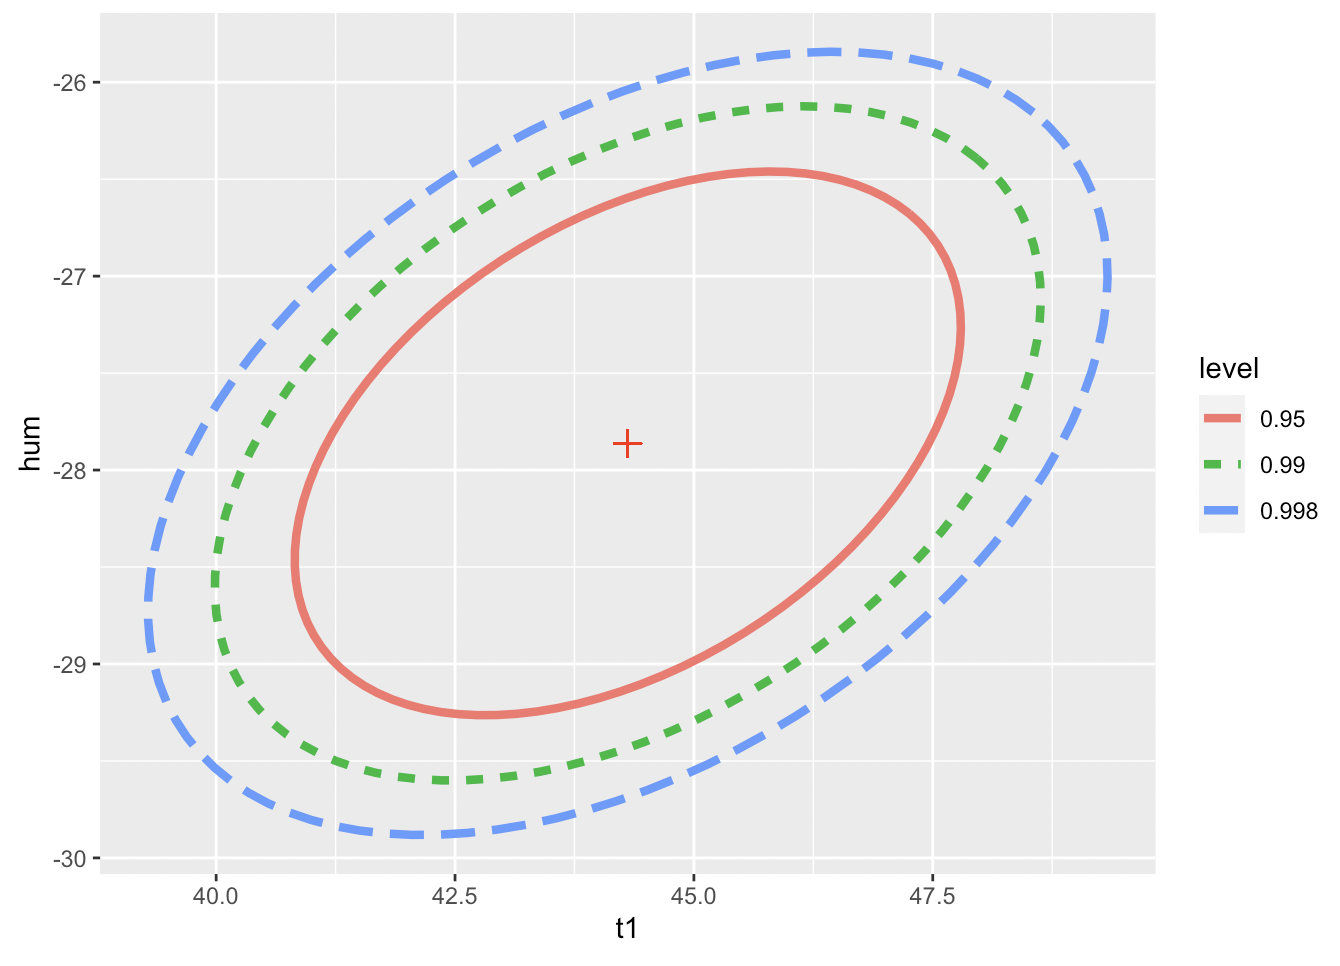
\includegraphics[scale=0.5]{9599998.png}
    \caption{}
    \label{}
\end{figure}\end{center}

\subsubsection{Confidence Interval for new observation}
\begin{lstlisting}[language=R]
x=data.frame(t(meanvalue))
predict.lm(bikeshare.mlr,x,interval="confidence",level=0.95)
##        fit      lwr      upr
## 1 1143.102 1129.198 1157.006
\end{lstlisting}
\subsubsection{Prediction Interval for new observation}
\begin{lstlisting}[language=R]
predict.lm(bikeshare.mlr,x,interval="prediction",level=0.95)
##        fit       lwr      upr
## 1 1143.102 -691.7461 2977.949
\end{lstlisting}

\subsection{Unusual Observation}
\subsubsection{Leverage Points}
\begin{lstlisting}[language=R]
lev=influence(bikeshare.mlr)$hat
# H matrix 的对角上的所有元素
newlev = lev[lev>2*p/n]
# 找出所有high leverage points
bikeshares.reg[lev > 2*p/n,]
# 筛选出bikeshares中high leverage points的项
\end{lstlisting}

\subsubsection{Half-norm Plot}
Designed to identify unusually large values and assess positive data.\\
Plot the data against the positive normal quantiles. Specifically,\\
1. Sort the data:
$$x_{[1]} \leq ... \leq x_{[n]}.$$
2. Compute the quantiles:
$$u_i=\Phi^{-1}(\frac{n+i}{2n+1})$$
3. Plot $x_{[i]}$ against $u_i$.
\begin{lstlisting}[language=R]
halfnorm(newlev, 6, labs=as.character(1:length(newlev)),
 ylab="Leverages")
# 6是nlab, 即给几个点标注
\end{lstlisting}
\begin{center}\begin{figure}[htbp]
  \centering
  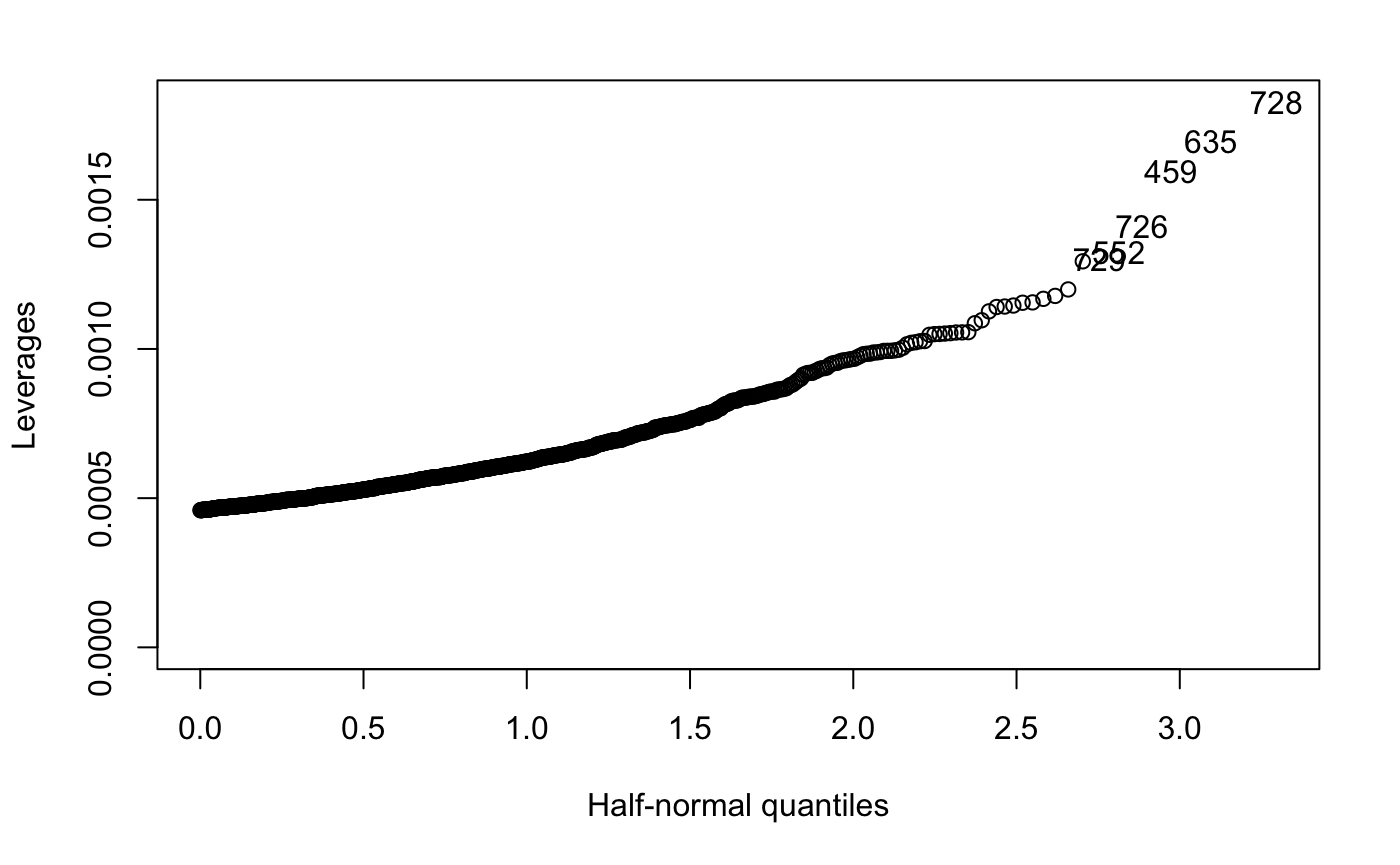
\includegraphics[scale=0.3]{week402.png}
  \caption{}
  \label{}
\end{figure}\end{center}




























\section{画图}

\subsection{$2\times2$的画布}
\begin{lstlisting}[language=R]
par(mfrow=c(2,2))
\end{lstlisting}
\subsection{plot点图,接上节 (bikeshares)}
\begin{lstlisting}[language=R]
par(mfrow=c(2,2))
# Plot of t1 vs. cnt
plot(bikeshares.reg$t1, bikeshares.reg$cnt, xlab="Real
Temperature in C", ylab="New Bike Shares")
# Plot of t2 vs. cnt
plot(bikeshares.reg$t2, bikeshares.reg$cnt, xlab=" Feels
Like Temperature in C", ylab="New Bike Shares")
# Plot of t1 vs. t2
plot(bikeshares.reg$t1, bikeshares.reg$t2, xlab=" Feels
Like Temperature in C", ylab="Real Temperature in C")
# Plot of hum vs. t1
plot(bikeshares.reg$hum, bikeshares.reg$t1, xlab="Humidity",
ylab="Real Temperature in C")
\end{lstlisting}
\begin{center}\begin{figure}[htbp]
    \centering
    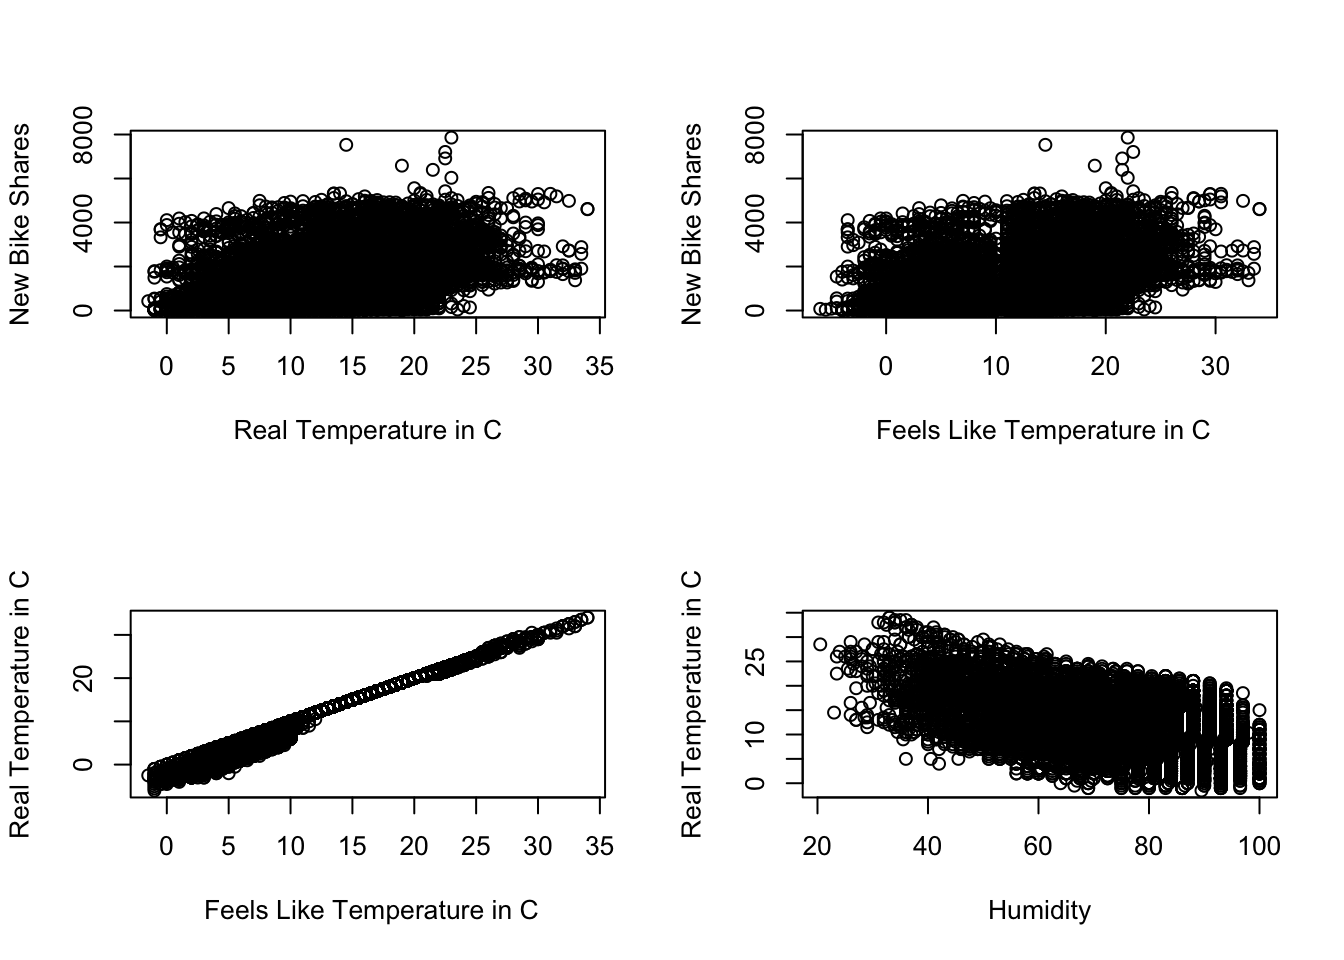
\includegraphics[scale=0.3]{Bike.png}
    \caption{}
    \label{}
\end{figure}\end{center}

\subsection{ggplot}
\begin{lstlisting}[language=R]
library(ggplot2)
\end{lstlisting}
\subsubsection{Plot the regression line along with the connected “point-wise” confidence intervals (galton)}
\begin{lstlisting}[language=R]
library(ggplot2)
ggplot(galton, aes(MP,AH)) + geom_point() + geom_smooth(method=lm)
\end{lstlisting}
\begin{center}\begin{figure}[htbp]
    \centering
    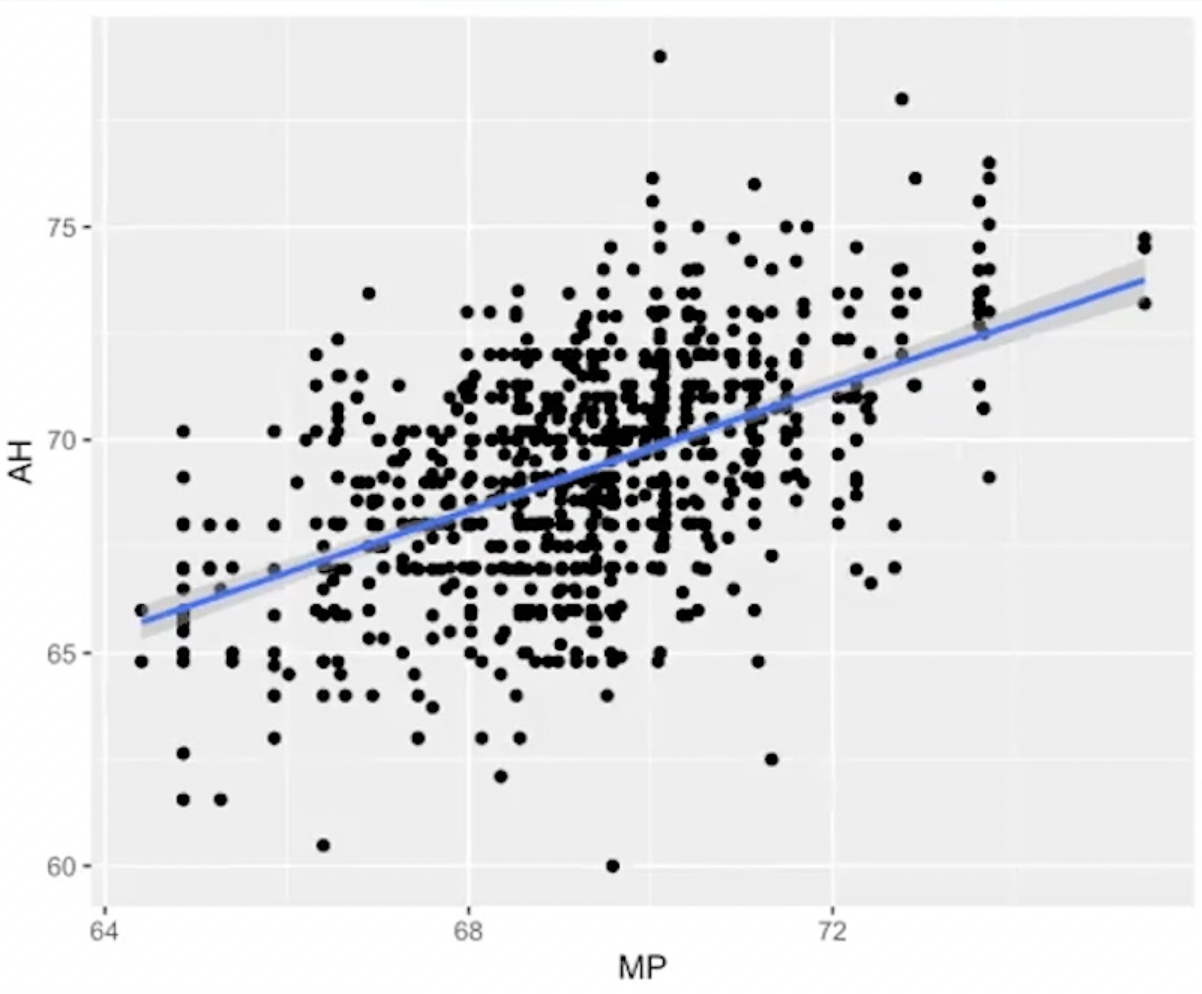
\includegraphics[scale=0.5]{plot1.png}
    \caption{}
    \label{}
\end{figure}\end{center}
\subsubsection{给颜色取名,竖直的线,坐标label}
\begin{lstlisting}[language=R]
# Form the data frame for plotting
ggplot(data=NULL, aes(x=0:56)) + 
  geom_line(aes(y=myCI[,1], colour="LSfit"), size=1) + 
  geom_line(aes(y=myCI[,2], colour="90% CI"), size=1) +
  geom_line(aes(y=myCI[,3], colour="90% CI"), size=1) +
  geom_line(aes(y=myPI[,2], colour="90% PI"), size=1, linetype=2)+
  geom_line(aes(y=myPI[,3], colour="90% PI"), size=1, linetype=2)+ 
  scale_colour_manual("", values=c("LSfit" = "black",
                               "90% CI" = "blue", 
                               "90% PI"="red"))+ 
  xlab("wind_speed") +ylab("bike shares")+ 
  geom_vline(xintercept = mean(bikeshares.reg$wind_speed),
  colour="purple", size=1, linetype=3)
\end{lstlisting}
\begin{center}\begin{figure}[htbp]
    \centering
    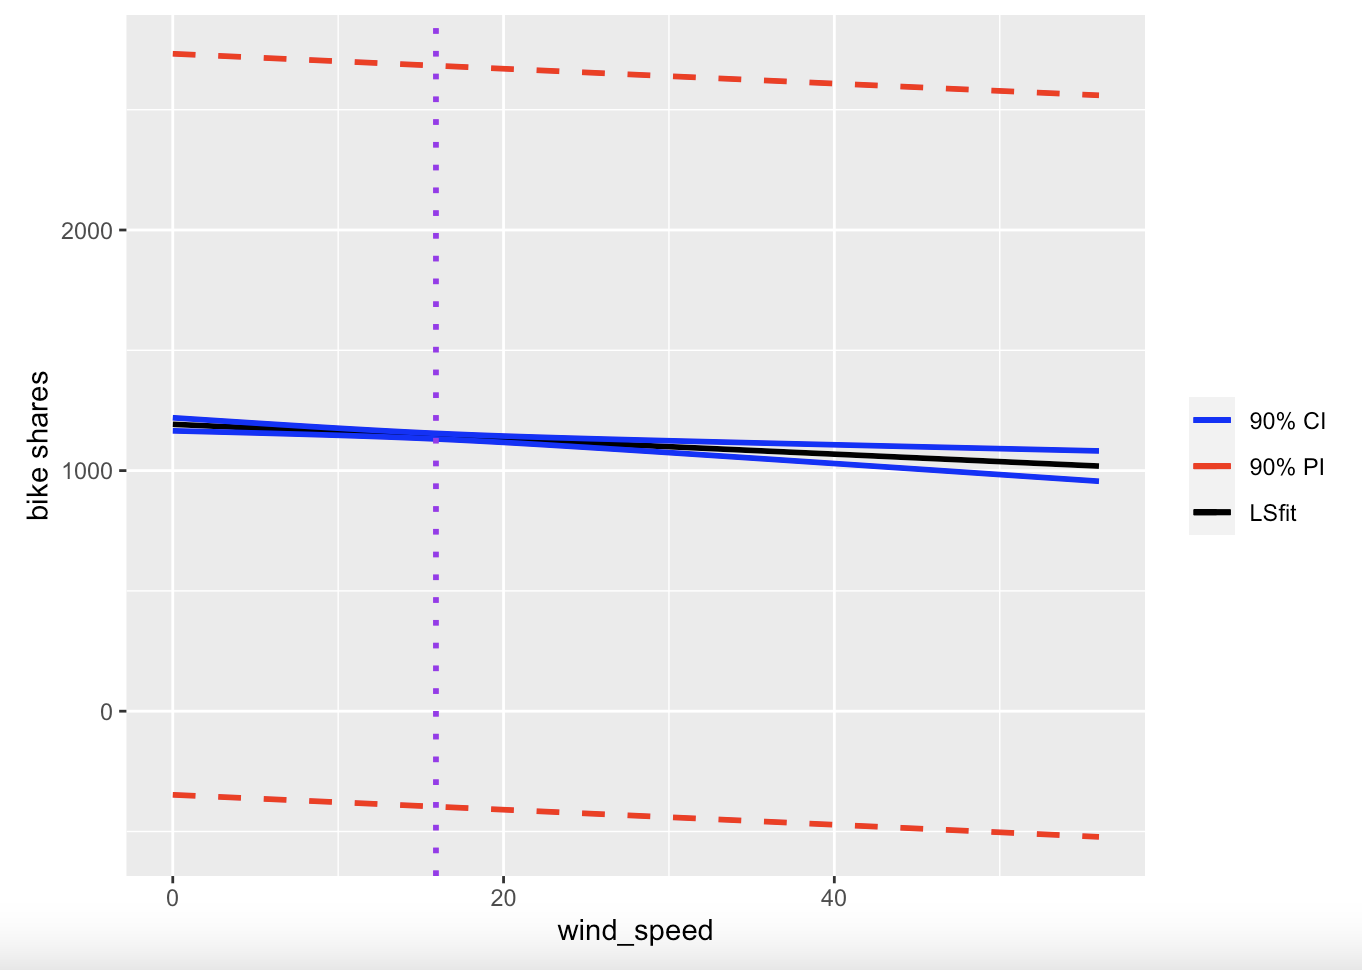
\includegraphics[scale=0.5]{week501.png}
    \caption{}
    \label{}
\end{figure}\end{center}

\end{document}